\subsection{Background}

\emph{DNA} is a chemical compound that contains the instructions for developing a living organism.
A \emph{gene} is a region of DNA that influences a particular characteristic of an individual.
An \emph{allele} is one possible form of a particular gene.
A \emph{chromosome} is a structure that holds a molecule of DNA\@.
The \emph{genotype} of an individual is its complete set of DNA, whereas its \emph{phenotype} is its observed characteristics.

\emph{Evolution} is the change in inherited traits of a population of organisms through successive generations.
This occurs when there is a change in the frequency of certain alleles in a population over time.
Evolution is caused by \emph{genetic variation} and \emph{natural selection}.

Genetic variation is caused by sexual reproduction, which can introduce new combinations of genes into a population, and mutation, which is a natural process that alters the DNA sequence of an individual, allowing variations that are not present in its parents.

Natural selection is the differential survival and reproduction of individuals due to differences in phenotype.
Some phenotypes may protect individuals from prey, or increase the likelihood of attracting mates, thereby increasing the chance of survival and reproduction.
Genotypes that are more likely to leave offspring are known as \emph{fitter} genotypes.
A genotype that is fit for one environment may not be fit for another.

In the case of an evolutionary algorithm, a fitter solution is one that has higher quality in terms of the objective function, and is, therefore, more likely to be used in the generation of new solutions.
After many iterations, solutions improve with respect to the objective function.

\subsection{Behaviour of an Evolutionary Algorithm}

In a population of candidate solutions, parent solutions are selected, recombined and mutated to produce offspring solutions.
Survivors are selected from the population for the next iteration.
The selection of parents and survivors is based on selective pressure towards fitter solutions.
There is a small chance that poor individuals survive to the next iteration.
Over many iterations, the population of solutions becomes more optimal.

Hill~climbing is a greedy local search algorithm that climbs from an initial solution to the nearest optimum.
Its solution can become trapped at a local optimum or a plateau.
Simulated~annealing is also a non-greedy local search algorithm.
It gives some probability towards accepting a worse solution.
The probability is initially high to allow exploration of the search space.
It decreases gradually to allow promising optima to be exploited.

Evolutionary algorithms maintain a population of candidate solutions rather than a single solution.
This helps to explore different regions of the search space.
The small probability of poor solutions being selected for recombination and survival helps to avoid local optima.
Evolutionary algorithms are global search algorithms.
They can generate new solutions that are not neighbours of current solutions.
One disadvantage of this is that some optima may not be visited.

\begin{figure}[!htp]
  \centering
  \caption*{Typical behaviour of an evolutionary algorithm.}
  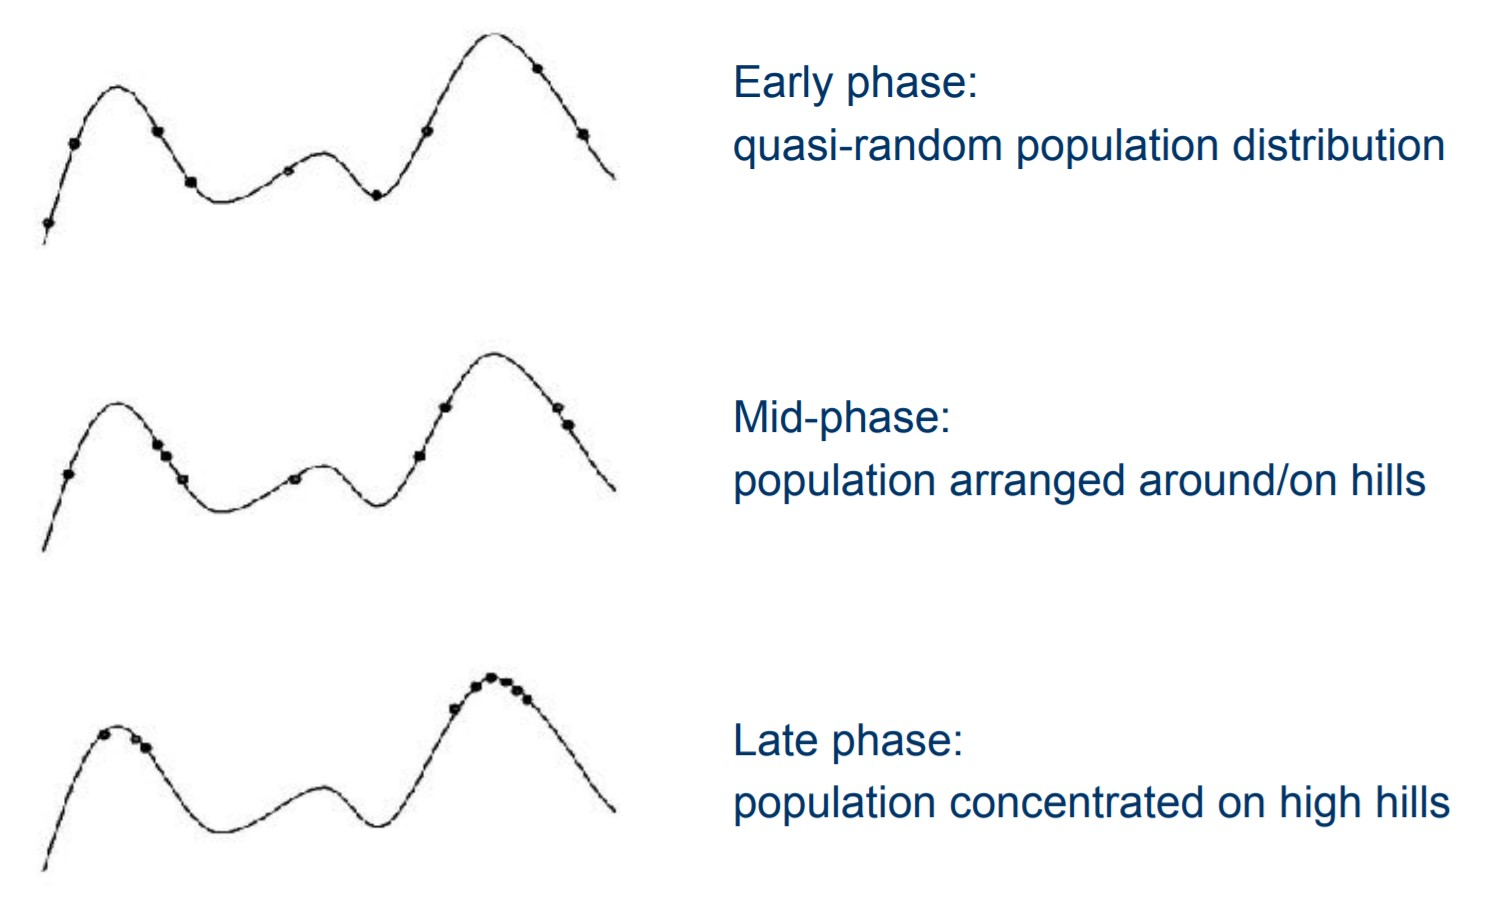
\includegraphics[width=0.6\textwidth]{unit-11/figures/phases.jpg}
\end{figure}

An evolutionary algorithm proceeds as follows.
\begin{enumerate}
  \item Initialise the population
  \item Evaluate the fitness of each solution
  \item Repeat until a termination condition is satisfied
  \begin{enumerate}
    \item Select parent solutions
    \item Recombine parent solutions with a probability \( P_{\mathrm{c}} \)
    \item Mutate resulting offspring with a probability \( P_{\mathrm{m}} \)
    \item Evaluate the fitness of each offspring solution
    \item Select survivors for the next iteration
  \end{enumerate}
\end{enumerate}
The selection of parents and survivors is based on selective pressure towards fitter solutions.

\subsection{Representation}

The representation of a candidate solution is its \emph{genotype} or \emph{encoding}.
The value of a solution is its \emph{phenotype}.
A phenotype that cannot be represented in the genotypic space cannot exist.
A representation must allow all feasible solutions to be represented.
It is useful for the representation to be easily manipulated by the algorithm.

Traditionally, a candidate solution for an evolutionary algorithm is represented as a \emph{binary~vector} or \emph{binary~string}.
Each position in the vector can assume a value of zero or one.
The genotypic space \( \left\{ 0, 1 \right\}^{L} \) is a binary~vector of length \( L \)\@.
Each position in the vector is a \emph{gene}.
The value of a gene is an \emph{allele}.

Integer vectors are useful for discrete, ordinal or categorical problems, floating-point vectors are useful for continuous problems, and matrices are useful for multidimensional problems such as staff allocation.

To \emph{encode} is to create a representation for a particular candidate solution.
To \emph{decode} is to recover the candidate solution from its representation.

It may be possible to encode a particular solution in more than one way using the representation, in which case, not all phenotypes would have the same chance of appearing in the initial population.
Nevertheless, a genotype or representation must decode to only one phenotype or candidate solution.

\subsection{Initialisation}

Initialisation is usually performed at random to ensure an even distribution of possible alleles.
One method of random initialisation is to initialise individual genes uniformly at random.
The initialisation process can make use of existing solutions or problem-specific heuristics to seed the population.
This increases the probability of generating initial solutions in regions that are more promising.

\subsection{Evaluation}

A \emph{fitness~function} assigns a value of fitness to each phenotype, and represents the requirements to which the population should adapt.
Often, the objective function is used as the fitness function.
The function may include strategies for dealing with constraints.
Typically, an evolutionary problem is formulated in terms of maximising fitness.
All minimisation problems can be formulated as maximisation problems.

\subsection{Parent Selection}

The selection of parent solutions is usually based on a probability such that
\begin{itemize}
  \item fitter solutions are more likely to be selected, and
  \item even the worst solutions have some chance of being selected.
\end{itemize}
The stochastic nature of parent selection helps to avoid solutions becoming trapped at local optima.

The number of parents to select is a design choice of the algorithm.
Commonly, the number of parents is chosen such that the number of offspring is equal to the current size of the population.
Two methods of parent selection are \emph{roulette wheel} and \emph{tournament} selection.

In roulette wheel selection, the probability of selection for an individual solution is proportional to its fitness.
The probability of selection for a solution \( a \), given a fitness function \( \function{f}{x} \) and that all solutions \( x \) belong to the current population \( X \), is given by
\begin{equation*}
  \frac{\function{f}{a}}{\sum_{x \in X} \function{f}{x}}
\end{equation*}
Since a parent must be selected from the current population, the probabilities for each candidate solution sum to one.

Disadvantages of roulette wheel selection are that
\begin{itemize}
  \item individual solutions of outstanding fitness may take over the population very quickly, causing \emph{premature convergence},
  \item when solutions have similar fitness, there is very little \emph{selective pressure}, and
  \item the mechanism behaves differently for transpositions of the fitness function that should result in the same solution.
\end{itemize}

In tournament selection, \( k \) solutions are picked from the population uniformly at random.
The selected parent is the fittest of these solutions.
This process is repeated to select more parents.
Tournament selection is able to apply selective pressure even when parents have similar fitness.

\subsection{Recombination}

Recombination is a process that generates offspring solutions based on parent solutions.
Recombination involving two parents is known as \emph{crossover}.
The recombination probability \( P_{\mathrm{c}} \) determines whether recombination occurs.
If it does not occur, the parents are cloned.
Most offspring will be similar or worse than their parents due to the random selection of parent genes.
Some offspring will be fitter, however.
\emph{Genetic algorithms} are evolutionary algorithms that have a high recombination probability, typically in the interval \( \left[ 0.6, 0.9 \right] \).

In \emph{single-point crossover}, a point between two positions in a representation vector is selected at random.
The parent solutions are split at the point, and their tails are exchanged.
The resulting crossovers are the children.

Single-point crossover has a number of disadvantages that arise from positional bias.
Its performance depends on the order that components of the design variable occur in the representation.
Adjacent genes are more likely to be kept together, and two genes from opposite ends of the vector can never be kept together.
This bias can be exploited if knowledge of the structure of the problem suggests that some genes should be kept together.

\emph{Multi-parent recombination} produces offspring from multiple parents using \emph{diagonal crossover}.
For \( k \) parents, \( k - 1 \) splitting points are selected.
Children are created from the split sections of their parents along diagonals.

\begin{table}[!htp]
  \centering
  \caption*{Diagonal crossover of three parents, each split into three sections A, B and C.}
  \begin{tabular}{ccccccc}
    \toprule
    \multicolumn{3}{c}{Parents} & & \multicolumn{3}{c}{Offspring} \\
    \midrule
    \textcolor{red}{A\textsubscript{1}} & \textcolor{blue}{B\textsubscript{1}} & \textcolor{green}{C\textsubscript{1}} & &
    \textcolor{red}{A\textsubscript{1}} & \textcolor{red}{B\textsubscript{2}} & \textcolor{red}{C\textsubscript{3}} \\
    \textcolor{green}{A\textsubscript{2}} & \textcolor{red}{B\textsubscript{2}} & \textcolor{blue}{C\textsubscript{2}} & &
    \textcolor{green}{A\textsubscript{2}} & \textcolor{green}{B\textsubscript{3}} & \textcolor{green}{C\textsubscript{1}} \\
    \textcolor{blue}{A\textsubscript{3}} & \textcolor{green}{B\textsubscript{3}} & \textcolor{red}{C\textsubscript{3}} & &
    \textcolor{blue}{A\textsubscript{3}} & \textcolor{blue}{B\textsubscript{1}} & \textcolor{blue}{C\textsubscript{2}} \\
    \bottomrule
  \end{tabular}
\end{table}

\emph{Intermediate recombination} for floating-point representations produces an offspring from the simple average of its parents.

\subsection{Mutation}

Mutation acts on one genotype and produces another.
This typically causes small changes to the solution.
It can introduce traits that did not originally exist in the population.

For binary vector representations, \emph{bitwise bit-flipping} is used.
Each gene (bit) is flipped with the probability \( P_{\mathrm{m}} \), which is known as the \emph{mutation rate}, and is typically in the interval
\begin{equation*}
  \left[ \frac{1}{\text{population size}}, \frac{1}{\text{genotype length}} \right]
\end{equation*}

For integer representations, \emph{random reset} or \emph{creep mutation} are used.
Random reset is most suitable for categorical design variables.
A new value is selected from the set of permissible values (excluding the current value) according to a discrete uniform distribution.
This means that each value has the same probability of selection.
Creep mutation is most suitable for ordinal design variables.
A new value is selected from the set of permissible values (excluding the current value) according to a discrete non-uniform distribution centred around the current value.
This can be achieved by adding a value from a binomial distribution to the current value and subtracting the mean of the distribution.

Uniform mutation for a floating-point representation is similar to a random reset.
A new value is selected from a continuous uniform distribution.
This means that each possible value has the same probability of selection.
Non-uniform mutation for a floating-point representation is similar to creep mutation.
The new value is generated using a continuous non-uniform distribution, such as a normal distribution.
This means that smaller changes are more likely than larger changes, and that an increase by a certain amount is equally as likely as a decrease by the same amount.

\subsection{Survival Selection}

Typically, solutions are selected for survival such that the population maintains a constant size.
The two main types of survival selection are \emph{age-based} and \emph{fitness-based}.

In age-based survival selection, all offspring solutions survive, and the previous generation dies.
The problem with this method is that fit solutions from the previous generation are lost.

One type of fitness-based survival selection is \emph{delete-worst} selection.
This removes the worst solutions from both the offspring and the previous generation, ensuring only the best solutions survive.
The problem with this method is that it can result in premature convergence.

Another type of fitness-based survival selection is \emph{elitism}, which is usually combined with age-based selection.
In general, all offspring survive, but if the offspring generation does not contain the best solution, the worst child is replaced by the best solution from the previous generation.

\subsection{Termination}

Commonly, the algorithm is terminated when
\begin{itemize}
  \item a maximum number of iterations is reached,
  \item a specified level of fitness is reached,
  \item a minimum level of diversity is reached, or
  \item a maximum number of iterations is reached without any improvement in fitness.
\end{itemize}

\subsection{Summary}

Evolutionary algorithms can be applied to a variety of optimisation problems.
Thus, it can be said that evolutionary algorithms are \emph{problem independent}.
Nevertheless, the choice of fitness function, constraint strategy, representation, initialisation, parent selection, recombination, mutation, survival selection and termination criteria depends on the problem.

\begin{description}
  \item[population] a multiset of individuals
  \item[individual] a candidate solution
  \item[genotype] the representation of a candidate solution
  \item[chromosome] the representation of a candidate solution
  \item[gene] a component of a chromosome
  \item[allele] the value of a gene
  \item[mutation] a unary variation operator that generates a new individual
  \item[crossover] a binary variation operator that generates one or more new individuals
  \item[recombination] an \( n \)-ary variation operator that generates one or more new individuals
  \item[fitness function] a function to be optimised by the evolutionary algorithm
  \item[generation] iteration
\end{description}
